\documentclass[10pt]{article}
\usepackage[margin=2cm]{geometry}
\usepackage{lipsum}
\usepackage{amsmath}
\usepackage[inline]{enumitem}
\usepackage{verbatim}
\usepackage{fancyvrb}
\usepackage{pgfornament}
\usepackage{amssymb, tabularx, xcolor, nccmath}
\usepackage[utf8]{inputenc}
\usepackage{cancel}
\usepackage[portuguese]{babel}
\usepackage{bbm}
\usepackage{titlesec}
\usepackage{setspace, mathtools}

\titleformat*{\section}{\sffamily\large\bfseries}
\titleformat*{\subsection}{\sffamily\normalsize\bfseries}
\makeatletter
\renewcommand*\env@matrix[1][\arraystretch]{%
  \edef\arraystretch{#1}%
  \hskip -\arraycolsep
  \let\@ifnextchar\new@ifnextchar
  \array{*\c@MaxMatrixCols c}}
\makeatother

\usepackage{hyperref}
\hypersetup{
    colorlinks=true,
    linkcolor=magenta,
    filecolor=magenta,      
    urlcolor=magenta,
}

\usepackage[T1]{fontenc}
\usepackage{ccfonts}
\renewcommand{\bfseries}{\fontfamily{cmbr}\fontseries{bx}\selectfont}
\DeclareMathAlphabet{\mathbf} {OT1}{cmbr}{bx}{n}
\DeclareMathAlphabet{\mathbold}{OML}{cmbrm}{b}{it}

\setlength{\parindent}{4em}
\setlength{\parskip}{1em}
\renewcommand{\baselinestretch}{1.2}


\def\changemargin#1#2{\list{}{\rightmargin#2\leftmargin#1}\item[]}
\let\endchangemargin=\endlist 



\DeclareMathOperator*{\argmin}{arg\,min}

\newcommand*{\QEDA}{\hfill\ensuremath{\blacksquare}}%
\newcommand*{\QEDB}{\hfill\ensuremath{\square}}%
\DeclareMathOperator*{\plim}{plim}

\setlength\parindent{0pt}

\usepackage{dsfont}

\newcommand\Z{\mathbf{Z}}
\newcommand\E{\mathbb{E}}

\newcommand\R{\mathbb{R}}
\newcommand\D{\mathbf{D}}
\newcommand\C{\mathbf{D}}
\newcommand\X{\mathbf{X}}
\newcommand\yy{\mathbf{y}}
\newcommand\ii{{\boldsymbol{\iota}}}
\renewcommand\O{{\boldsymbol{\Omega}}}
\newcommand\y{\mathbf{y}}
\newcommand\e{\mathbf{e}}
\renewcommand\u{\mathbf{u}}
\renewcommand\d{\mathbf{d}}
\newcommand\resid{\mathbf{u}}
\newcommand\0{\mathbf{0}}
\newcommand\betabold{\pmb{\beta}}
\newcommand\ones{\boldsymbol{\iota}}
\newcommand\epbold{\boldsymbol{\epsilon}}
\newcommand\varep{\boldsymbol{\varepsilon}}
\newcommand\x{\mathbf{x}}
\newcommand\z{\mathbf{z}}
\newcommand\Q{\mathbf{Q}}
\newcommand\I{\mathbf{I}}
\newcommand\w{{\mathbf{w}}}
\newcommand\wm{\bar{\mathbf{w}}}
\newcommand\M{{\mathbf{M}}}
\renewcommand\P{{\mathbf{P}}}
\newcommand\var{\operatorname{var}}
\newcommand\cov{\operatorname{cov}}
\renewcommand\b{\mathbf{b}}
\renewcommand\e{\mathbf{b}}


\usepackage{amssymb,graphicx}
\def\tallqed{\smash{\scalebox{.75}[1.025]{\color{blue!50!black}$\blacksquare$}}}

\tolerance=1
\emergencystretch=\maxdimen
\hyphenpenalty=10000
\hbadness=10000

\newcommand{\prnt}[1]{\ensuremath{\left(#1\right)}} %parentheses
\newcommand{\colch}[1]{\ensuremath{\left[#1\right]}} %square brackets
\newcommand{\chave}[1]{\ensuremath{\left\{#1\right\}}}  %curly brackets

\usepackage{stackengine}
\renewcommand\useanchorwidth{T}
\usepackage{graphicx}
\stackMath

\allowdisplaybreaks

\usepackage{MnSymbol}

\newcommand{\mytext}[1]% #1 = same as intertext
{&\parbox{0.94\textwidth}{\rule{0pt}{.5\baselineskip}\\
\textrm{#1}\\
\rule{0pt}{.5\baselineskip}}&\\}

\newcounter{exercise}
\newcounter{problem}[exercise]
\newcommand{\myitem}{\stepcounter{problem}\tag*{\alph{problem})}}

\usepackage{amsmath, amsthm, amssymb, amsfonts, enumitem, fancyhdr, color, comment, graphicx, environ, csquotes}


\newenvironment{problem}[2][Problem]{\begin{trivlist}
\item[\hskip \labelsep {\bfseries #1}\hskip \labelsep {\bfseries #2.}]}{\end{trivlist}}
\newenvironment{sol}
    {\\[1em] {\color{magenta}\text{Resposta.}}
    }
    {{\color{blue!50!black}\QEDA}}

\setlength{\parskip}{\baselineskip}%

\usepackage[framed,numbered,autolinebreaks,useliterate]{mcode}
\lstset{breakatwhitespace=false} %%<---this line added
\usepackage{listings}
\lstset{
        language=Matlab,
        breaklines=true
    }
    
\begin{document}

\stepcounter{exercise}
\newdimen\headerwidth


\begin{center}
  \framebox{
    \vbox{
      \headerwidth=\textwidth
      \vspace{1mm}
      \advance\headerwidth by -0.22in
      \hbox to \headerwidth {\it Doutorado em Economia - EPGE/FGV \hfill MDPEMF024 - Métodos Numéricos}
      \vspace{5mm}
      \hbox to \headerwidth {{\Large \hfill Lista \#1 \hfill}}
      \vspace{6mm}
      \hbox to \headerwidth {\hfill \today \hfill}
      \vspace{5mm}
      \hbox to \headerwidth {{\it Aluno: Rafael Vetromille  \hfill Professor: Cézar Santos / TA: Ana Paula Ruhe}}
      \vspace{1mm}
      }
    }
\end{center}

\textbf{Informações}: Para essa lista, você trabalhará com o seguinte processo estocástico AR(1):
\begin{align*}
z_t = \rho z_{t-1} + \varepsilon_t
\end{align*}
com $\varepsilon_t \sim N(0, \sigma^2)$. Assuma, por enquanto, que $\rho = 0.95$ e $\sigma = 0.007$, calibração de Cooley and Prescott (1995).

\section*{Questão \#1}

Discretize o processo acima usando o método de Tauchen (1986). Use
9 pontos.
\begin{sol}
O código a seguir representa uma das possibilidades de se implementar o método de Tauchen no \verb|Matlab|. No código em anexo, as funções estão no final do arquivo \verb|.m|. Primeiramente, definimos um vetor de zeros e uma matriz diagonal para depois alocarmos os valores que serão obtidos. Agora devemos determinar a imagem do grid, a localização e o número de pontos. O ``upper bound'' será definido como $\theta_N$ e será igual a 
\begin{align*}
\theta_N = + m \times \sqrt{\frac{\sigma^2}{1-\rho^2}}
\end{align*}  
em que $\sigma(\sqrt{1-\rho^2})^{-1}$ é o desvio padrão incondicional de $\theta$ e $m$ é um parâmetro de escala. O limite inferior, por sua vez, será definido como
\begin{align*}
\theta_1 = - m \times \sqrt{\frac{\sigma^2}{1-\rho^2}}
\end{align*}
Os demais $N-2$ pontos do grid serão calculados de forma equidistantes entre $\theta_1$ e $\theta_N$, isto é, cada passo poderá ser calculado como:
\begin{align*}
\texttt{step} = \frac{\theta_N - \theta_1}{N-1}
\end{align*}
e podemos fazer um for loop para calcular os $N-2$ pontos restantes, conforme descrito nas linhas 15 a 17 do código abaixo.

Em seguida, precisamos saber qual é a probabilidade de passar para o estado $\theta_j$ condicional de estar no estado $\theta_i$ com $i, j \in [1,2, \ldots, N]$ em que $N$ represente o número de pontos no grid. Para tanto, denote esta probabilidade por $p_{i,j }= P(\theta_{t+1} = \theta_{j} \mid \theta_t = \theta_i)$ e seja $P$ a matriz de $\{p_{i,j}\}^{N,N}_{i=1,j=1}$. A abordagem de Tauchen discretiza a distribuição de probabilidade condicional.

Suponha que o estado atual seja $\theta_i$ . Qual é a probabilidade de se mover para $\theta_j$? Após algumas contas, podemos calculá-la da seguinte forma: 
\begin{align*}
p_{i,j} = \Phi\left(\frac{\theta_j + \Delta \theta / 2 - \rho \theta_i}{\sigma}\right) - \Phi\left(\frac{\theta_j - \Delta \theta / 2 - \rho \theta_i}{\sigma}\right)
\end{align*}
A transição para os pontos do canto deve ser tratada de forma diferente
\begin{align*}
p_{i,1} = \Phi\left(\frac{\theta_1 + \Delta \theta / 2 - \rho \theta_i}{\sigma}\right) \quad \land \quad p_{i,N} = 1 - \Phi\left(\frac{\theta_N - \Delta \theta / 2 - \rho \theta_i}{\sigma}\right)
\end{align*}
Agora, podemos calcular as probabilidades de transição $p_{i,j}$
para todo $i$ e $j$. O resultado desta discretização é um grid $\{\theta_i\}^N_{i=1}$ e a matriz de probabilidade de transição $P$. A função no quadro abaixo implementa exatamente esse algoritmo e retorna os dois objetos da discretização:

\lstinputlisting[firstline=261, lastline=295]{matlab/lista1.m}

Agora, podemos aplicar a função anterior e obter os resultados da discretização. Antes disso, precisamos definir as variáveis calibradas, o número de estados e o parâmetro de escala (ad-hoc). Assim, temos:
\newpage
\lstinputlisting[firstline=1, lastline=30]{matlab/lista1.m}
Nesse código, as variáveis \verb|S9T| e \verb|P9T| representam o grid de estados ($N \times 1$) e a matriz de transição ($N\times N$) obtida pelo método de Tauchen, respectivamente. O resultado via Matlab (\%.4f) obtido será:
\begin{lstlisting}
S9T =

   -0.0673   -0.0504   -0.0336   -0.0168         0    0.0168    0.0336    0.0504    0.0673

P9T =

    0.7644    0.2347    0.0009    0.0000    0.0000         0         0         0         0
    0.0592    0.7405    0.1997    0.0006    0.0000    0.0000         0         0         0
    0.0001    0.0747    0.7569    0.1679    0.0004    0.0000    0.0000         0         0
    0.0000    0.0001    0.0931    0.7669    0.1396    0.0002    0.0000    0.0000         0
    0.0000    0.0000    0.0002    0.1147    0.7702    0.1147    0.0002    0.0000         0
    0.0000    0.0000    0.0000    0.0002    0.1396    0.7669    0.0931    0.0001    0.0000
    0.0000    0.0000    0.0000    0.0000    0.0004    0.1679    0.7569    0.0747    0.0001
    0.0000    0.0000    0.0000    0.0000    0.0000    0.0006    0.1997    0.7405    0.0592
    0.0000    0.0000    0.0000    0.0000    0.0000    0.0000    0.0009    0.2347    0.7644
\end{lstlisting}
\end{sol}


\section*{Questão \#2}

Discretize o processo acima usando o método de Rouwenhorst. Use 9
pontos.
\begin{sol}
O método de Rouwenhorst, recentemente reintroduzido por Kopechy and Suen (RED, 2010), não depende da discretização da distribuição condicional de $\theta$. O algoritmo pode ser descrito da seguinte forma:  \vspace{-0.4cm}
\begin{enumerate}[wide]
\item Escolha o tamanho do grid e defina esse tamanho como $N$. Agora,  calcule seus pontos finais da seguinte forma: 
\begin{align*}
\theta_N = + \sigma_\theta\times  \sqrt{N-1} \quad \land \quad \theta_1 = - \sigma_\theta \times \sqrt{N-1}
\end{align*}
onde  $\sigma_\theta^2 = {\sigma^2}/{(1-\rho^2)}$.
\item Agora, calcule a matriz de transição de forma recursiva da seguinte forma: 
\begin{align*}
P = p \times \begin{bmatrix}
P_{N-1} & \0 \\
\0' & 0
\end{bmatrix} + (1-p) \times \begin{bmatrix}
\0 & P_{N-1}  \\
0 & \0'
\end{bmatrix} + (1-p) \times \begin{bmatrix}
\0' & 0 \\
P_{N-1} & \0
\end{bmatrix} + p \times \begin{bmatrix}
0 & \0' \\
\0 & P_{N-1} 
\end{bmatrix}
\end{align*}
onde \mcodefn{p  = (1+rho)/2}, \mcodefn{P2 = [p 1-p; 1-p p]} e $\0$ é um vetor coluna de zeros de dimensão $(N-1)\times 1$.
\item Normalize as linhas para somarem 1.
\end{enumerate}
\vspace{-0.3cm}
A função a seguir representa uma das formas de implementar o método de Rouwenhorst no \verb|Matlab|: \vspace{-0.4cm}
\lstinputlisting[firstline=297, lastline=325]{matlab/lista1.m} \vspace{-0.3cm}
Agora, podemos aplicar a função anterior e obter os resultados da discretização. Note que já definimos as variáveis calibradas no início do código e, portanto, não precisaríamos repetir, mas para fins didáticos coloquei a calibração novamente. O número de estados continua a ser $N=9$. Assim, temos:
\vspace{-0.4cm}
\lstinputlisting[firstline=34, lastline=56]{matlab/lista1.m} \vspace{-0.3cm}
Nesse código, as variáveis \verb|S9R| e \verb|P9R| representam o grid de estados ($N \times 1$) e a matriz de transição ($N\times N$) obtida pelo método de Rouwenhorst, respectivamente. O resultado via Matlab (\%.4f) obtido será:
\vspace{-0.4cm}
\begin{lstlisting}
S9R =

   -0.0634   -0.0476   -0.0317   -0.0159    0.0000    0.0159    0.0317    0.0476    0.0634

P9R =

    0.8167    0.1675    0.0150    0.0008    0.0000    0.0000    0.0000    0.0000    0.0000
    0.0209    0.8204    0.1469    0.0113    0.0005    0.0000    0.0000    0.0000    0.0000
    0.0005    0.0420    0.8231    0.1261    0.0081    0.0003    0.0000    0.0000    0.0000
    0.0000    0.0016    0.0630    0.8247    0.1051    0.0054    0.0001    0.0000    0.0000
    0.0000    0.0001    0.0032    0.0841    0.8253    0.0841    0.0032    0.0001    0.0000
    0.0000    0.0000    0.0001    0.0054    0.1051    0.8247    0.0630    0.0016    0.0000
    0.0000    0.0000    0.0000    0.0003    0.0081    0.1261    0.8231    0.0420    0.0005
    0.0000    0.0000    0.0000    0.0000    0.0005    0.0113    0.1469    0.8204    0.0209
    0.0000    0.0000    0.0000    0.0000    0.0000    0.0008    0.0150    0.1675    0.8167
\end{lstlisting}
\end{sol}
\section*{Questão \#3}

Simule o processo contínuo para 10000 períodos. Faça o mesmo para os
processos discretizados (lembre-se de usar as mesmas realizações para
os choques). Compare os caminhos para cada processo (gráficos serão
úteis aqui). Se eles não estiverem muito próximos, utilize mais pontos.
\begin{sol}
Primeiramente, implementemos a função que simula o AR(1) no Matlab. Nesse caso, colocamos \mcodefn{Z[0] = 0} (estado inicial), simulamos um vetor aleatório com $T = 10000$ observações obtido de uma distribuição normal com a função \mcodefn{normrnd()} com parâmetros $\sigma = 0.007$ e $\mu = 0$.  A seguinte função implementa o processo:
\lstinputlisting[firstline=327, lastline=336]{matlab/lista1.m}
O resultado pode ser obtido utilizando-se a função acima da seguinte forma:
\lstinputlisting[firstline=60, lastline=82]{matlab/lista1.m}
O comando \mcodefn{rnd(1234)} tem por objetivo deixar o código replicável para outros usuários obterem sempre os mesmos resultados. Essa função tem como \textit{output} dois vetores como descrito no comentário. 

Para retornarmos a simulação para os processos discretizados, primeiramente criamos um vetor chamado \mcodefn{idx} que alocará todos os índices do vetor de estados \mcodefn{theta}, isto é, a posição no vetor $N\times 1$. Após isso, definimos o estado inicial. O primeiro estado (estado inicial) é simplesmente a mediana, pois o grid é centrado na média e tem $N = 9$ elementos que é um número ímpar. Agora, para cada período dos $T = 10000$ choques simulados, registramos a probabilidade de ir para o primeiro estado. Após isso, percorremos cada um dos estados do grid discreto (via colunas da matriz) da seguinte forma: pegamos a linha da matriz de transição do espaço de estado anterior e verificamos quais colunas (índices) a CDF do choque \mcodefn{i} é menor do que a probabilidade acumulada obtida pela soma acumulada das linhas da matriz de transição com a função \mcodefn{cum = cumsum(Pi')';} e, por fim, salvamos o primeiro elemento do vetor resultante. Esse será o nosso próximo estado, podendo permanecer no mesmo ou mudar. No Matlab, uma forma de implementar esse código é da seguinte maneira:
\lstinputlisting[firstline=338, lastline=349]{matlab/lista1.m}
O resultado será o vetor \mcodefn{idx} com $10000$ elementos dos índices do vetor de estados. Para obtermos esse resultado basta rodarmos as seguintes linhas de código:
\lstinputlisting[firstline=192, lastline=201]{matlab/lista1.m}
As últimas duas linhas transformam os vetores \mcodefn{IDXT} (posição dos estados do grid obtido pelo método de Tauchen) e \mcodefn{IDXR} (posição dos estados do grid obtido pelo método de Rouwenhorst) nos valores de fato que os estados assumem. Podemos ver os primeiros dez resultados  de ambos os métodos discretizados da seguinte maneira:
\begin{lstlisting}
>> AR1D_T95(1:10)

ans =

         0         0         0         0    0.0168    0.0168    0.0168    0.0336    0.0336    0.0336

>> AR1D_R95(1:10)

ans =

     0     0     0     0     0     0     0     0     0     0
\end{lstlisting}
Agora, comparando os caminhos via gráfico (veja o código para gerar os gráficos abaixo no documento \mcodefn{lista1.m}), temos:
\begin{figure}[htp!]
\centering
	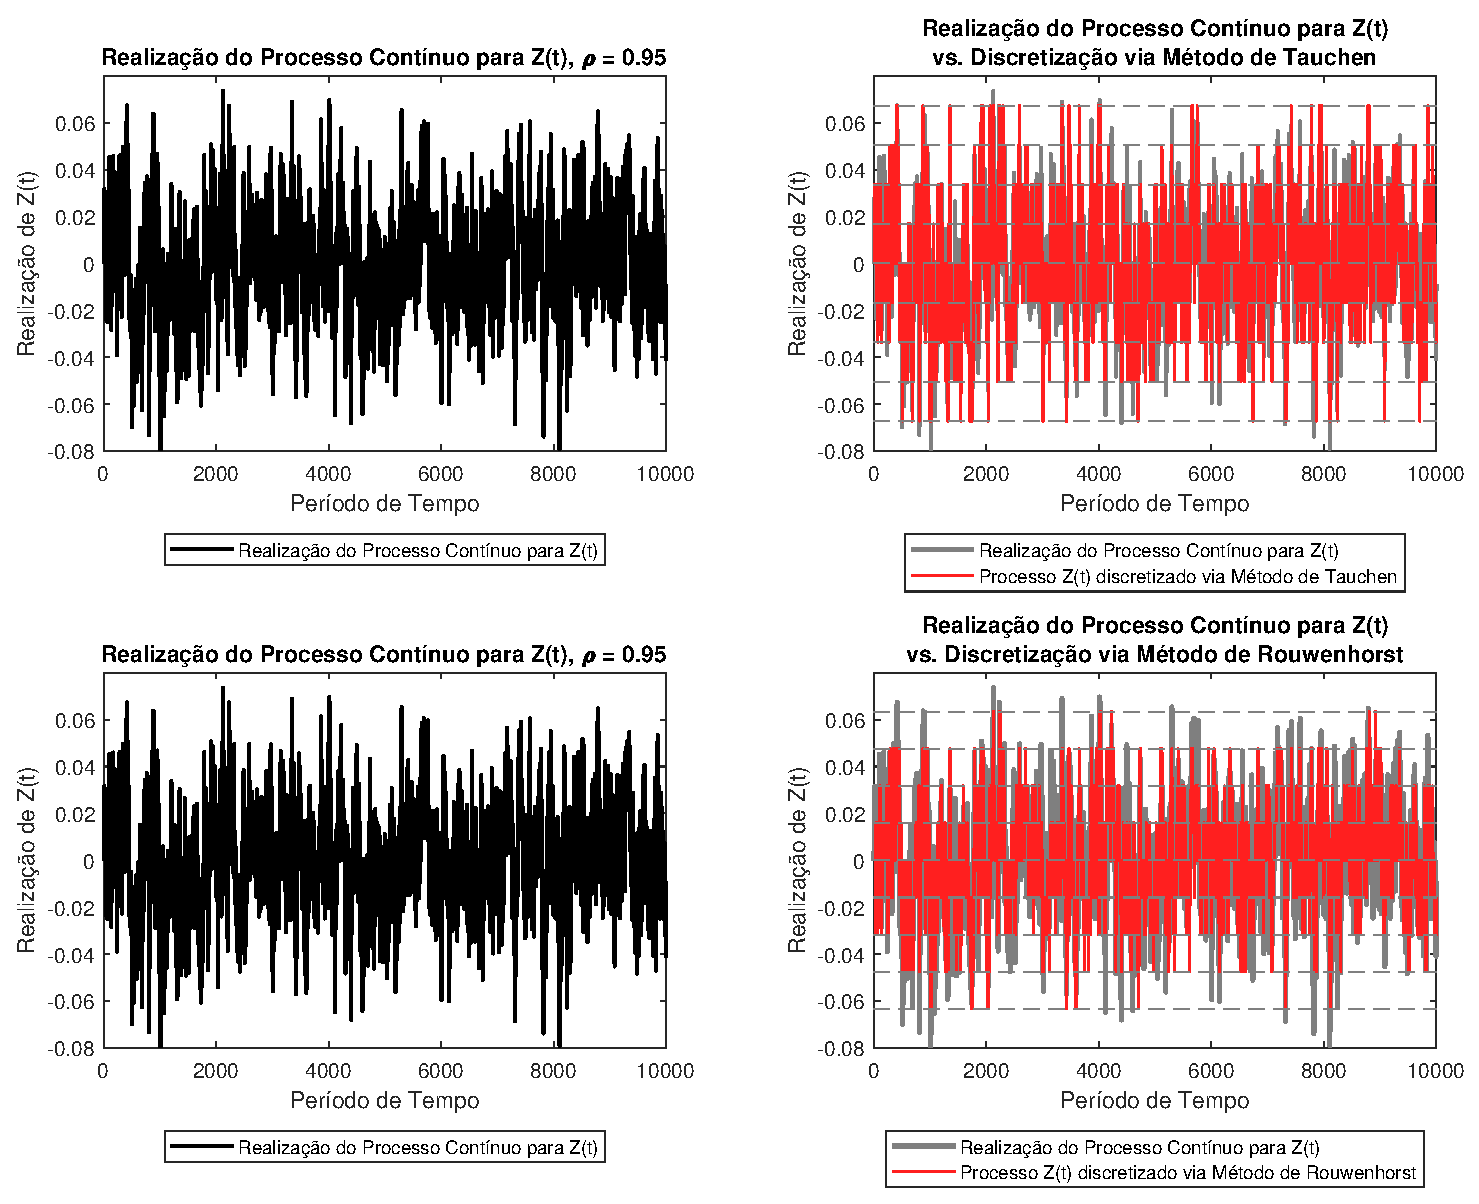
\includegraphics[scale=0.63]{myfig.eps}
\end{figure}

Note que o processo discretizado estão relativamente próximos do processo contínuo. Uma forma melhor de comparar isso graficamente seria se o exercício pedisse um $T$ menor. Dessa forma, conseguiríamos comparar com maior precisão.
\end{sol}

\newpage

\section*{Questão \#4}

Estime processos AR(1) com base nos dados simulados, tanto a partir
do Tauchen quanto o de Rouwenhorst. Quão próximo eles estão do
processo gerador de dados real? Se eles não estiverem muito próximos,
utilize mais pontos.
\begin{sol}
Para estimarmos bastar utilizarmos a função \mcodefn{fitlm} para rodar a regressão e a função \mcodefn{lagmatrix} para calular o lag da variável dependente. Assim, temos: \vspace{-0.2cm} 
\lstinputlisting[firstline=149, lastline=155]{matlab/lista1.m}
O resultado obtido é: \vspace{-0.2cm}
\begin{lstlisting}
>> lm1_95

lm1_95 = 

Linear regression model:
    y ~ x1

Estimated Coefficients:
          Estimate       SE        tStat     pValue
          ________    _________    ______    ______

    x1    0.95239     0.0030497    312.29      0   

Number of observations: 9999, Error degrees of freedom: 9998
Root Mean Squared Error: 0.00814

>> lm2_95

lm2_95 = 

Linear regression model:
    y ~ x1

Estimated Coefficients:
          Estimate       SE        tStat     pValue
          ________    _________    ______    ______

    x1    0.95339     0.0030187    315.83      0   

Number of observations: 9999, Error degrees of freedom: 9998
Root Mean Squared Error: 0.00693
\end{lstlisting}
Note que em ambas as regressões os valores do coeficiente defasado é bem próximo de 0.95. No entanto, o mais correto é considerar o erro padrão pois não estamos trabalhando com estimativa pontual e sim intervalar. Nesse caso, podemos rodar um teste de hipótese $H_0: \rho = 0.95$ vs. $H_1: \rho \neq 0.95$. Assim, a estatística do teste pode ser calculada como: 
\begin{align*}
t_{\text{calc}} = \frac{\hat{\beta}_{\text{OLS}} - 0.95}{\text{ep}(\hat{\beta}_{\text{OLS}})}
\end{align*}
No Matlab, podemos computá-las da seguinte maneira:
\begin{lstlisting}
% Compute t-statistic
tStat_tauchen = (lm1_95.Coefficients.Estimate - 0.95)/lm1_95.Coefficients.SE;
tStat_rouwenh = (lm2_95.Coefficients.Estimate - 0.95)/lm2_95.Coefficients.SE;
\end{lstlisting}
Os resultados obtidos, serão:
\begin{lstlisting}
>> tStat_tauchen

tStat_tauchen =

    0.7844

>> tStat_rouwenh

tStat_rouwenh =

    1.1215
\end{lstlisting}
Ambos menores que o valor crítico de 1.96. Logo, não rejeitamos a nula. E, portanto, devemos ter cuidado na interpretação desse resultado. Se simularmos 100 processos AR(1) e discretizá-los via método de Tauchen ou Rouwenhorst, o parâmetro verdadeiro $\rho = 0.99$ pertencerá a 95 deles. 
\end{sol}

\newpage

\section*{Questão \#5}

Refaça os exercícios acima quando $\rho = 0.99$. 

\begin{enumerate}[label = 5.\arabic*., wide]

\item Discretize o processo acima usando o método de Tauchen (1986). Use
9 pontos.
\begin{sol}
No Matlab, temos o seguinte: \vspace{-0.4cm}
\lstinputlisting[firstline=159, lastline=170]{matlab/lista1.m}
O resultado será: \vspace{-0.4cm}
\begin{lstlisting}
S9T =

   -0.1489   -0.1116   -0.0744   -0.0372    0.0000    0.0372    0.0744    0.1116    0.1489


P9T =

    0.9928    0.0072    0.0000         0         0         0         0         0         0
    0.0024    0.9914    0.0062    0.0000         0         0         0         0         0
    0.0000    0.0028    0.9918    0.0054    0.0000         0         0         0         0
    0.0000    0.0000    0.0033    0.9921    0.0046    0.0000         0         0         0
    0.0000    0.0000    0.0000    0.0039    0.9921    0.0039    0.0000         0         0
    0.0000    0.0000    0.0000    0.0000    0.0046    0.9921    0.0033    0.0000         0
    0.0000    0.0000    0.0000    0.0000    0.0000    0.0054    0.9918    0.0028    0.0000
    0.0000    0.0000    0.0000    0.0000    0.0000    0.0000    0.0062    0.9914    0.0024
         0    0.0000    0.0000    0.0000    0.0000    0.0000    0.0000    0.0072    0.9928
\end{lstlisting}
\end{sol}

\item Discretize o processo acima usando o método de Rouwenhorst. Use 9
pontos.
\begin{sol}
No Matlab, temos o seguinte: \vspace{-0.4cm}
\begin{lstlisting}
% Re-calibration
rho      = 0.99;                         
sig      = 0.007;         
N        = 9;        % Number of points (states);  

% Rouwenhorst's method
[S9R, P9R] = rouwenhorst(rho, sig, N)
\end{lstlisting}
O resultado será: \vspace{-0.4cm}
\begin{lstlisting}
S9R =

   -0.1404   -0.1053   -0.0702   -0.0351         0    0.0351    0.0702    0.1053    0.1404


P9R =

    0.9607    0.0386    0.0007    0.0000    0.0000    0.0000    0.0000    0.0000    0.0000
    0.0048    0.9609    0.0338    0.0005    0.0000    0.0000    0.0000    0.0000    0.0000
    0.0000    0.0097    0.9610    0.0290    0.0004    0.0000    0.0000    0.0000    0.0000
    0.0000    0.0001    0.0145    0.9611    0.0241    0.0002    0.0000    0.0000    0.0000
    0.0000    0.0000    0.0001    0.0193    0.9611    0.0193    0.0001    0.0000    0.0000
    0.0000    0.0000    0.0000    0.0002    0.0241    0.9611    0.0145    0.0001    0.0000
    0.0000    0.0000    0.0000    0.0000    0.0004    0.0290    0.9610    0.0097    0.0000
    0.0000    0.0000    0.0000    0.0000    0.0000    0.0005    0.0338    0.9609    0.0048
    0.0000    0.0000    0.0000    0.0000    0.0000    0.0000    0.0007    0.0386    0.9607
\end{lstlisting}
\end{sol}

\item Simule o processo contínuo para 10000 períodos. Faça o mesmo para os
processos discretizados (lembre-se de usar as mesmas realizações para
os choques). Compare os caminhos para cada processo (gráficos serão
úteis aqui). Se eles não estiverem muito próximos, utilize mais pontos.
\begin{sol}
Igualmente ao item 3, temos:  
\lstinputlisting[firstline=179, lastline=201]{matlab/lista1.m}
\newpage
Graficamente (veja o código do gráfico no arquivo \mcodefn{lista1.m}), temos:
\begin{figure}[htp!]
\centering
	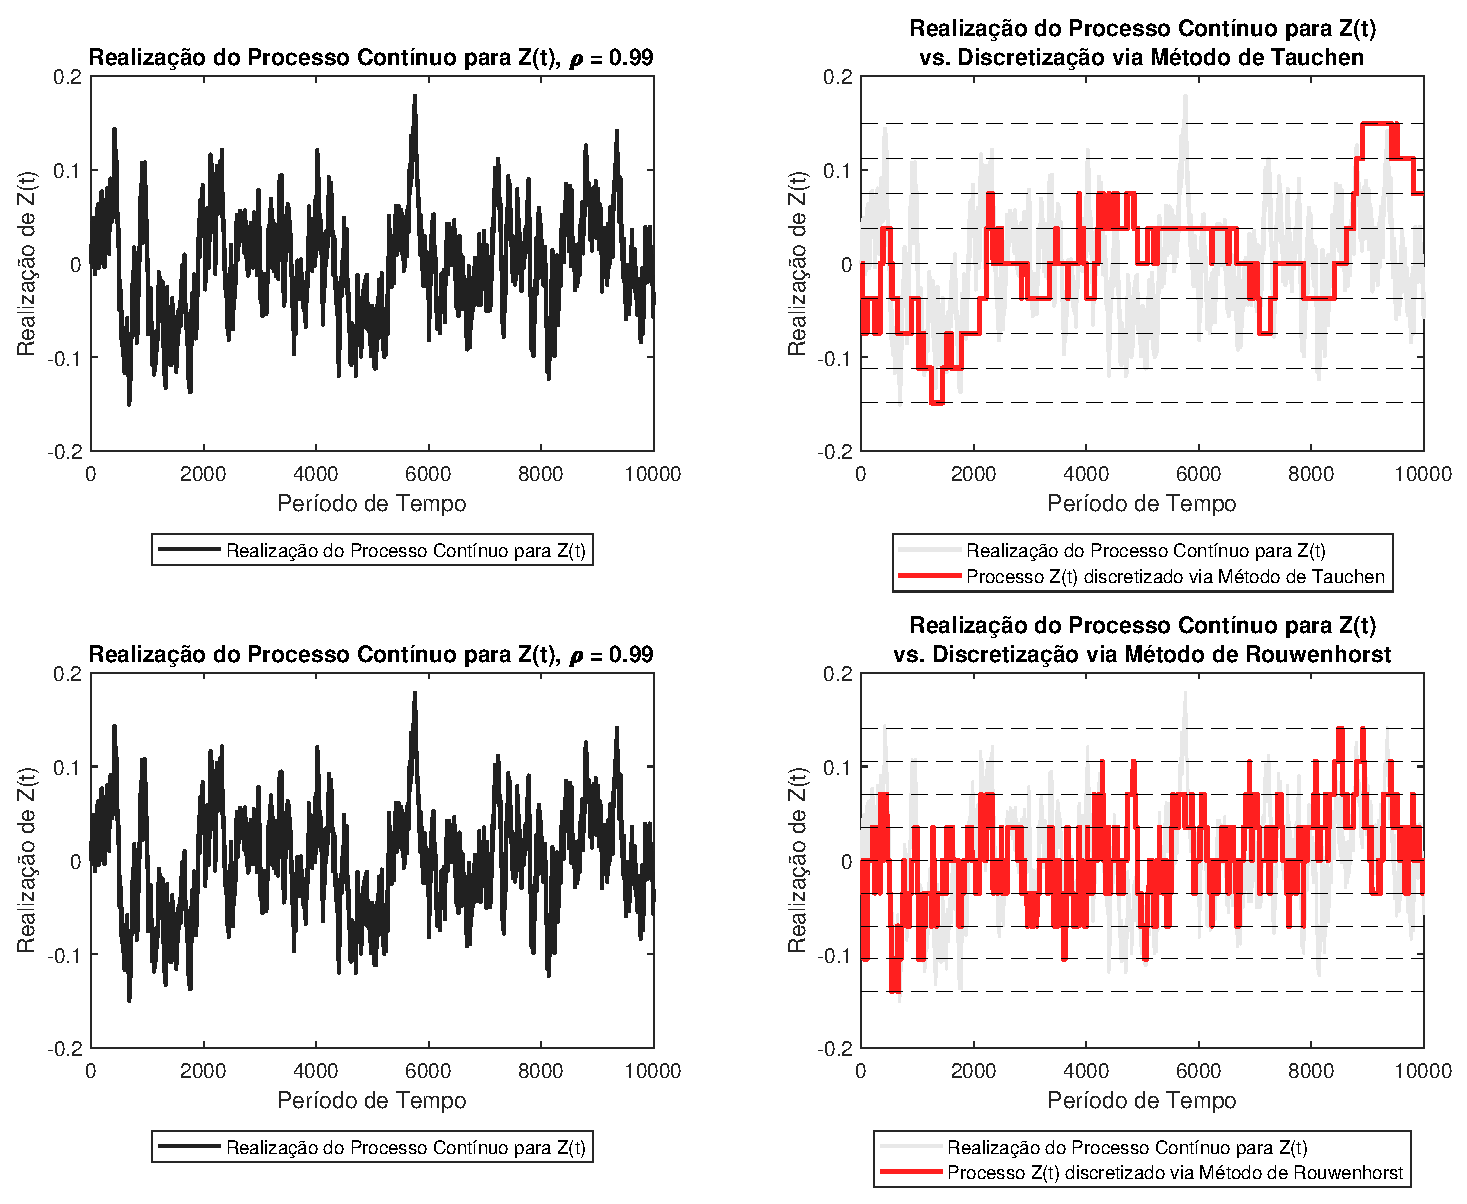
\includegraphics[scale=0.63]{myfig1.eps}
\end{figure}\\
Note que quando $\rho = 0.99$, a discretização via método de Tauchen fica muito ruim, enquanto que a discretização via método de Rouwenhorst aproxima melhor o processo contínuo, conforme evidenciado por Kopecky e Suen (2010). Sendo assim, quando há uma maior persistência do choque, isto é, quando $\rho$ se aproxima de 1, o método de Rouwenhorst torna-se mais confiável.
\end{sol}
\item Estime processos AR(1) com base nos dados simulados, tanto a partir
do Tauchen quanto o de Rouwenhorst.
\begin{sol}
Igualmente ao item 4, temos: 
\begin{lstlisting}
% For simplicity, let's call the variables as Y1 (Tauchen) and Y2 (Rouwenhorst)
Y1 = AR1D_T99;
Y2 = AR1D_R99;

% Run the regressions
lm1_99 = fitlm(lagmatrix(Y1,1), Y1, 'Intercept', false);
lm2_99 = fitlm(lagmatrix(Y2,1), Y2, 'Intercept', false);

% Compute t-statistic (hyphotesis test)
tStat_tauchen = (lm1_99.Coefficients.Estimate - 0.99)/lm1_99.Coefficients.SE;
tStat_rouwenh = (lm2_99.Coefficients.Estimate - 0.99)/lm2_99.Coefficients.SE;
\end{lstlisting}
\newpage
O resultado das regressões pode ser conferido abaixo: \vspace{-0.4cm}
\begin{lstlisting}
>> lm1_99

lm1_99 = 

Linear regression model:
    y ~ x1

Estimated Coefficients:
          Estimate        SE        tStat     pValue
          ________    __________    ______    ______

    x1    0.99876     0.00051122    1953.7      0   


Number of observations: 9999, Error degrees of freedom: 9998
Root Mean Squared Error: 0.00333
>> lm2_99

lm2_99 = 

Linear regression model:
    y ~ x1

Estimated Coefficients:
          Estimate       SE        tStat     pValue
          ________    _________    ______    ______

    x1    0.99046     0.0013801    717.69      0   


Number of observations: 9999, Error degrees of freedom: 9998
Root Mean Squared Error: 0.00676
\end{lstlisting}
Já o resultado dos testes de hipóteses nos dizem que: \vspace{-0.4cm}
\begin{lstlisting}
>> tStat_tauchen

tStat_tauchen =

   17.1319

>> tStat_rouwenh

tStat_rouwenh =

    0.3327
\end{lstlisting}
Note que o teste de hipóteses que testa a nula $H_0: \rho = 0.99$ para o método de Tauchen rejeita a hipótese nula (\mcodefn{abs(tStat_tauchen) >=  1.96}), enquanto que o método de Rouwenhorst não rejeita (\mcodefn{abs(tStat_tauchen) < 1.96}). Isso indica que ao simularmos 100 processos contínuos e discretizarmos via ambos os métodos, no método de Tauchen 95 intervalos não conterão o parâmetro $\rho$ verdadeiro, enquanto que no método de Rouwenhorst 95 intervalos conterão o parâmetro $\rho$ verdadeiro.

Note que se aumentarmos o grid para $N = 15$, a discretização via método de Tauchen fica bem melhor. Graficamente, temos:
\begin{figure}[htp!]
\centering
	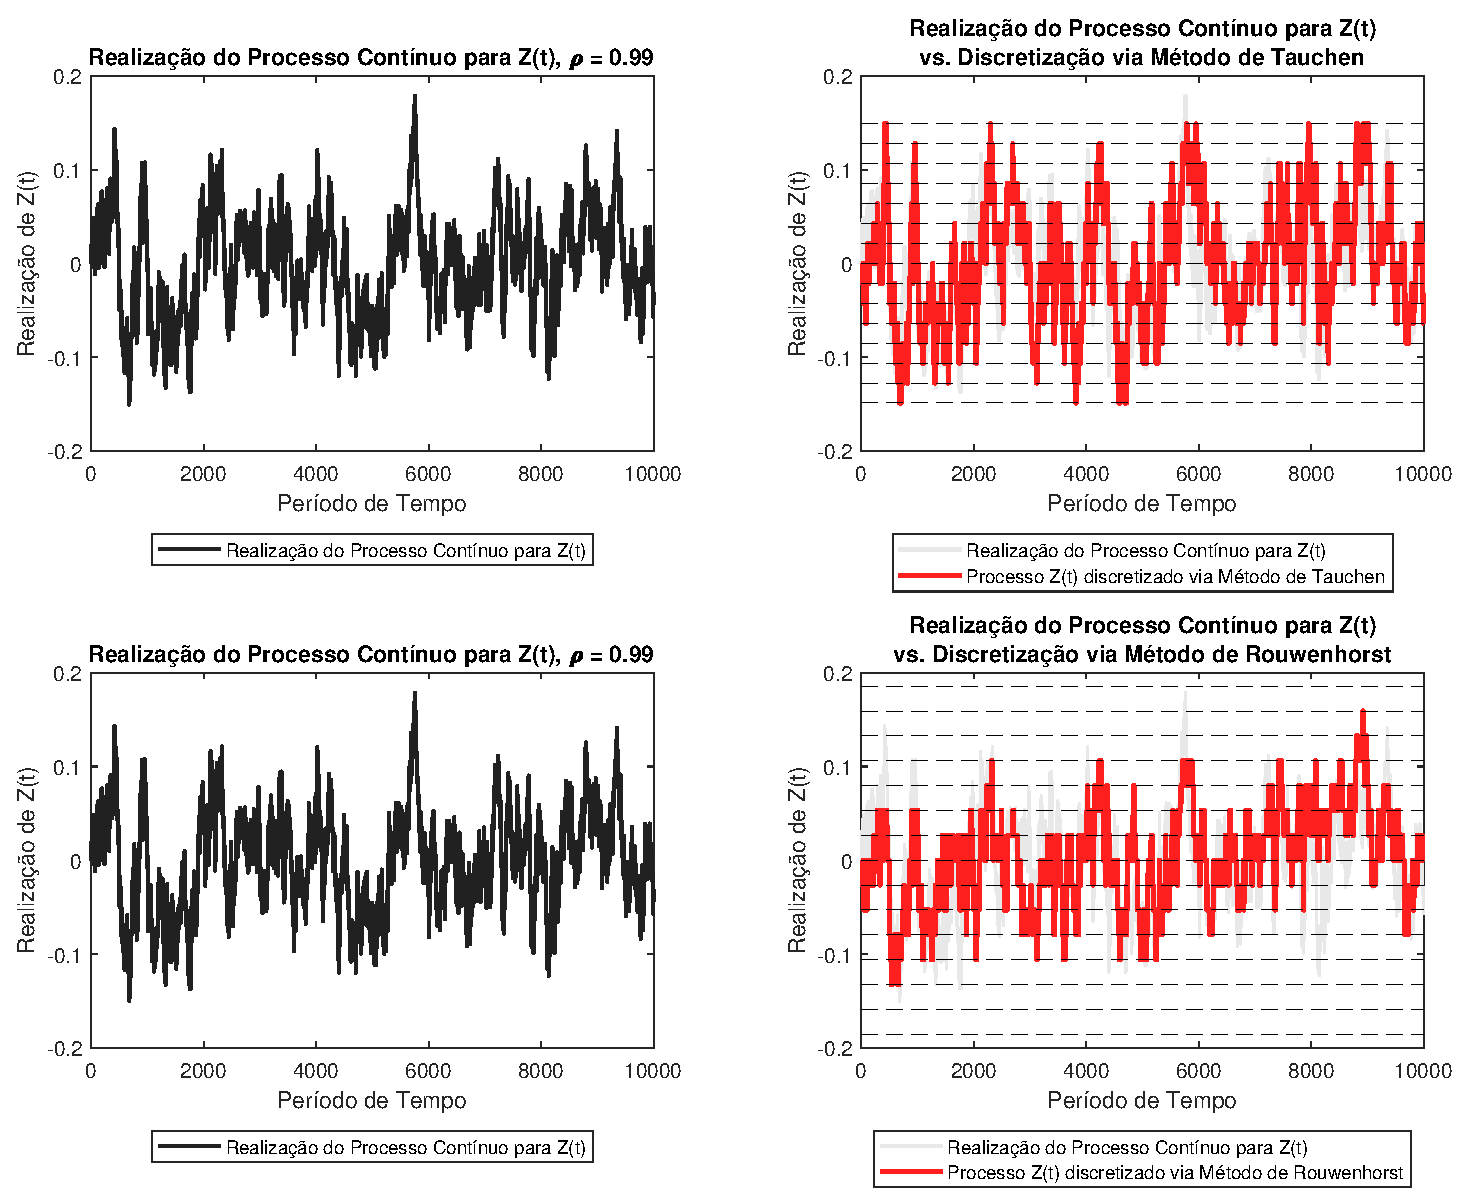
\includegraphics[scale=0.63]{myfig2.eps}
\end{figure}\\
Agora na regressão, a estatísitica t será: 
\begin{lstlisting}
>> tStat_tauchen

tStat_tauchen =

    2.5875

>> tStat_rouwenh

tStat_rouwenh =

    1.1073
\end{lstlisting}
ou seja, continuamos a rejeitar a hipótese nula com o método de Tauchen.
\end{sol}
\end{enumerate}




\end{document}
